\documentclass[11pt]{article}
\usepackage[utf8]{inputenc}
\usepackage[T1]{fontenc}
\usepackage[french]{babel}
\usepackage[top=1.8cm, bottom=1.8cm, left=1.8cm, right=1.8cm]{geometry}
\usepackage[linktocpage,colorlinks=false]{hyperref}
\usepackage{graphicx}
\usepackage{epsfig}
\usepackage{amssymb}
\usepackage{amsmath}
\usepackage{array}
\usepackage{subfig}
\usepackage{multicol}
\usepackage{caption}
\usepackage{algorithm}
\usepackage{color}
\usepackage{algorithmic}
\usepackage{listings}
\usepackage{url}
\usepackage{fullpage}
\usepackage{color}
\usepackage[table]{xcolor}
\usepackage{listings}

\definecolor{darkWhite}{rgb}{0.94,0.94,0.94}

\lstset{
	aboveskip=3mm,
	belowskip=-2mm,
	backgroundcolor=\color{darkWhite},
	basicstyle=\footnotesize,
	breakatwhitespace=false,
	breaklines=true,
	captionpos=b,
	commentstyle=\color{gray},
	deletekeywords={...},
	escapeinside={\%*}{*)},
	extendedchars=true,
	framexleftmargin=16pt,
	framextopmargin=3pt,
	framexbottommargin=6pt,
	frame=tb,
	keepspaces=true,
	keywordstyle=\color{blue},
	language=C,
	literate=
	{²}{{\textsuperscript{2}}}1
	{⁴}{{\textsuperscript{4}}}1
	{⁶}{{\textsuperscript{6}}}1
	{⁸}{{\textsuperscript{8}}}1
	{€}{{\euro{}}}1
	{é}{{\'e}}1
	{è}{{\`{e}}}1
	{ê}{{\^{e}}}1
	{ë}{{\¨{e}}}1
	{É}{{\'{E}}}1
	{Ê}{{\^{E}}}1
	{û}{{\^{u}}}1
	{ù}{{\`{u}}}1
	{â}{{\^{a}}}1
	{à}{{\`{a}}}1
	{á}{{\'{a}}}1
	{ã}{{\~{a}}}1
	{Á}{{\'{A}}}1
	{Â}{{\^{A}}}1
	{Ã}{{\~{A}}}1
	{ç}{{\c{c}}}1
	{Ç}{{\c{C}}}1
	{õ}{{\~{o}}}1
	{ó}{{\'{o}}}1
	{ô}{{\^{o}}}1
	{Õ}{{\~{O}}}1
	{Ó}{{\'{O}}}1
	{Ô}{{\^{O}}}1
	{î}{{\^{i}}}1
	{Î}{{\^{I}}}1
	{í}{{\'{i}}}1
	{Í}{{\~{Í}}}1,
	morekeywords={*,...},
	numbers=left,
	numbersep=10pt,
	numberstyle=\tiny\color{black},
	rulecolor=\color{black},
	showspaces=false,
	showstringspaces=false,
	showtabs=false,
	stepnumber=1,
	stringstyle=\color{black},
	tabsize=4,
	title=\lstname,
}



\hypersetup{
    colorlinks=true,
    breaklinks=true,
    urlcolor=red,
}
\parskip=5pt

\title{\huge{\textbf Calcul sécurisé - Attaque par faute sur DES}}
\author{CAUMES Clément 21501810}
\date{Master 1 Informatique SeCReTs \\ \url{www.github.com/Heisenberk/DFA-DES}}

\begin{document}

\maketitle
\vspace{20em}
%\begin{center}\includegraphics{pictures/Application.png}\end{center}
\newpage

\tableofcontents
\newpage

\section{Partie 1 : Attaque par faute sur le DES}

Une attaque par faute consiste à changer le résultat d'un sous calcul afin d'obtenir une information secrète. Ce changement va donc produire volontairement une erreur. Cette attaque est physique car, pour modifier la valeur de certains bits, il est nécessaire d'agir physiquement sur les composants électroniques. 
Dans le cas du DES avec une attaque par faute sur la valeur de sortie $R_{15}$ du $15^{e}$ tour, cela signifie que la valeur $R_{15}$ va être changer par l'attaquant. 

\begin{center}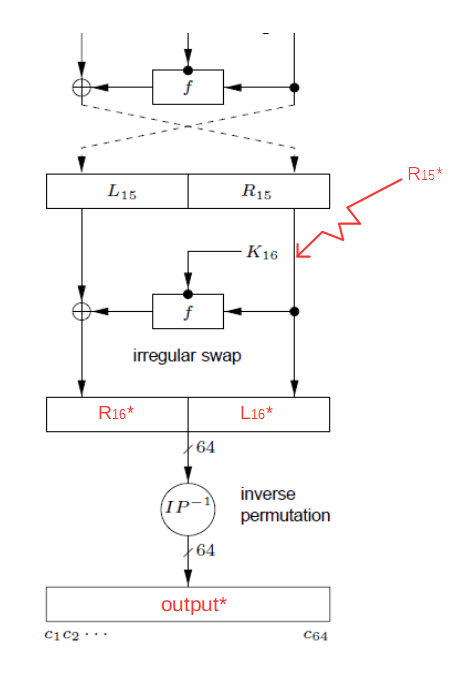
\includegraphics[scale=0.6]{../pictures/fauteR15.png}\end{center}

A partir de cette attaque, il est possible de retrouver la clé secrète utilisée par la victime à partir de la sous clé $K_{15}$. On suppose ici que nous sommes l'attaquant et que nous avons réussi à obtenir de la victime le message clair associé à son message chiffré (avec une clé inconnue pour le moment, qui est à trouver). De plus, nous avons eu de la victime 32 chiffrés (toujours avec la même clé) et dont on a réussi à faire une attaque par faute. Ainsi, pour mener correctement à bien cette attaque, il faut trouver $K_{16}$ puis en déduire $K$. Le détail de cette attaque sera montré par la suite. \newpage

\section{Partie 2 : Application concrète}

\subsection{Question 1}

Cette attaque par faute sur le dernier tour du DES comporte plusieurs étapes : 

\begin{itemize}
	\item étape 1 : trouver $R_{15}$ à partir du chiffré juste et les $R_{15}*$ à partir des chiffrés faux. \newline Pour cela, on fait une permutation initiale (qui annule la permutation finale $IP^{-1}$) pour trouver $L_{16}$ et $R_{16}$. On fera de même pour $R_{15}*$ à partir des chiffrés faux. On peut désormais écrire les formules suivantes : \newline \newline $R_{16}= L_{15} \oplus f(K_{16}, R_{15})$ et $L_{16}=R_{15}$ pour le chiffré juste. 
	\newline $R_{16}*= L_{15} \oplus f(K_{16}, R_{15}*)$ et $L_{16}*=R_{15}*$ pour les chiffrés faux. \newline \newline Le but ici est d'obtenir $K_{16}$ : pour cela, on fait le XOR entre $R_{16}$ et un $R_{16}*$. Ce qui nous donne l'équation suivante : \newline \newline
	$R_{16} \oplus R_{16}* =  L_{15} \oplus f(K_{16}, R_{15}) \oplus L_{15} \oplus f(K_{16}, R_{15}*)$ \newline 
	%\newline \Leftrightarrow g$
	Les $L_{15}$ s'annulent et on obtient : $R_{16} \oplus R_{16}* = f(K_{16}, R_{15}) \oplus f(K_{16}, R_{15}*)$ \newline \newline
	Or, $f(K_{i+1}, R_{i})=P(S(E(R_{i})\oplus K_{i+1})) = P(S_1(E(R_i)\oplus K_{i+1})_{b_1\to b_6} || ... || S_8(E(R_i)\oplus K_{i+1})_{b_{43}\to b_{48}})$ \newline
		
	\item étape 2 : pour chaque chiffré faux (associé à son $R_{15}*$), établir 8 équations pour chaque boîte-S. \newline
	
	$P^{-1}(R_{16}\oplus R_{16}*)_{b_1\to b_4} = S_1(E(R_{15})\oplus K_{16})_{b_1\to b_4} \oplus S_1(E(R_{15}*)\oplus K_{16})_{b_1\to b_4}$
	
	$P^{-1}(R_{16}\oplus R_{16}*)_{b_5\to b_{8}} = S_2(E(R_{15})\oplus K_{16})_{b_5\to b_{8}} \oplus S_2(E(R_{15}*)\oplus K_{16})_{b_5\to b_{8}}$
	
	$P^{-1}(R_{16}\oplus R_{16}*)_{b_{9}\to b_{12}} = S_3(E(R_{15})\oplus K_{16})_{b_{9}\to b_{12}} \oplus S_3(E(R_{15}*)\oplus K_{16})_{b_{9}\to b_{12}}$
	
	$P^{-1}(R_{16}\oplus R_{16}*)_{b_{13}\to b_{16}} = S_4(E(R_{15})\oplus K_{16})_{b_{13}\to b_{16}} \oplus S_4(E(R_{15}*)\oplus K_{16})_{b_{13}\to b_{16}}$
			
	$P^{-1}(R_{16}\oplus R_{16}*)_{b_{17}\to b_{20}} = S_5(E(R_{15})\oplus K_{16})_{b_{17}\to b_{20}} \oplus S_5(E(R_{15}*)\oplus K_{16})_{b_{17}\to b_{20}}$
				
	$P^{-1}(R_{16}\oplus R_{16}*)_{b_{21}\to b_{24}} = S_6(E(R_{15})\oplus K_{16})_{b_{21}\to b_{24}} \oplus S_6(E(R_{15}*)\oplus K_{16})_{b_{21}\to b_{24}}$
					
	$P^{-1}(R_{16}\oplus R_{16}*)_{b_{25}\to b_{28}} = S_7(E(R_{15})\oplus K_{16})_{b_{25}\to b_{28}} \oplus S_7(E(R_{15}*)\oplus K_{16})_{b_{25}\to b_{28}}$
						
	$P^{-1}(R_{16}\oplus R_{16}*)_{b_{29}\to b_{32}} = S_8(E(R_{15})\oplus K_{16})_{b_{29}\to b_{32}} \oplus S_8(E(R_{15}*)\oplus K_{16})_{b_{29}\to b_{32}}$ \newline
	
	\item étape 3 : éliminer les équations dont $P^{-1}(R_{16}\oplus R_{16}*)_{b_x\to b_y}$ vaut $0$, ainsi que celle dont $S_z(E(R_{15})\oplus K_{16})_{b_{x}\to b_{y}} = S_z(E(R_{15}*)\oplus K_{16})_{b_{x}\to b_{y}}$ puisqu'elles n'apporteront aucune information sur la portion de sous clé $K_{16}$. \newline
	
	\item étape 4 : faire une attaque exhaustive sur la sortie de chaque boîte-S de \newline $S_z(E(R_{15})\oplus K_{16})_{b_{x}\to b_{y}}$ : pour chaque élément, on déduit les possibles valeurs d'entrée de la boîte-S $E(R_{15})\oplus K_{16}$. (En effet, avec la configuration non linéaire des boîtes-S, on a 4 valeurs d'entrée possibles par valeur de sortie.) Ainsi, on en déduit une possible $K_{16}$. \newline
	
	\item étape 5 : pour chaque $K_{16}$ possible, calculer $S_z(E(R_{15}*)\oplus K_{16})_{b_{x}\to b_{y}}$ et regarder si \newline $P^{-1}(R_{16}\oplus R_{16}*)_{b_{x}\to b_{y}} = S_z(E(R_{15})\oplus K_{16})_{b_{x}\to b_{y}} \oplus S_z(E(R_{15}*)\oplus K_{16})_{b_{x}\to b_{y}}$. Si c'est le cas, alors $K_{16}$ en question devient une portion de clé candidate pour le chiffré faux associé. \newline
	
	\item étape 6 : Pour chaque boîte-S, il y a une liste de clés candidates pour chaque chiffré faux qui agit sur la portion de sous clé. Trouver pour chaque boîte-S l'intersertion des portions de clés candidates. Il y aura donc 1 portion de clé (sur 6 bits) par boîte-S. \newline
	
	\item étape 7 : concaténer les $8 \times 6$ bits pour obtenir la sous clé $K_{16}$. \newline
	
	La complexité pour trouver $K_{16}$ correspond à la recherche exhaustive de l'étape 4 : \newline $O(32 \times 8 \times 2^4 \times 4)$ car pour chaque chiffré faux (dans notre cas $32$), on regarde pour chaque boîte-S ($8$ dans le DES) les 4 entrées possibles (1 sortie vaut 4 entrées différentes dans une boîte-S). \newline Donc on a une complexité de $O(2^5 \times 2^3 \times 2^4 \times 2^2)=O(2^{14})$ pour trouver $K_{16}$. 

\end{itemize}

\subsection{Question 2}

Après avoir implémenter les fonctions "$attack\_sbox$", "$find\_intersection$" et "$find\_K16$" du fichier $app/src/attack.c$ fournis en annexe, on obtient pour chaque boîte-S les résultats suivants : 

\begin{enumerate}
	\item Boîte-S 1 : 
	\begin{itemize}
		\item Chiffré faux 1 : $\color{blue}0$ $4$ $5$ $10$ $14$ $19$ $20$ $24$ $25$ $30$ $34$ $39$ $\longrightarrow$ $12$ portions de sous clés possibles
		\item Chiffré faux 28 : $\color{blue}0$ $1$ $4$ $5$ $a$ $b$ $16$ $17$ $24$ $25$ $34$ $35$ $\longrightarrow$ $12$ portions de sous clés possibles
		\item Chiffré faux 29 : $\color{blue}0$ $2$ $5$ $7$ $\longrightarrow$ $4$ portions de sous clés possibles
		\item Chiffré faux 30 : $\color{blue}0$ 1 4 5 9 d 20 23 24 27 $\longrightarrow$ 10 portions de sous clés possibles
		\item Chiffré faux 31 : $\color{blue}0$ 8 24 2c $\longrightarrow$ 4 portions de sous clés possibles
		\item Chiffré faux 32 : $\color{blue}0$ e 10 1e 20 30 $\longrightarrow$ 6 portions de sous clés possibles \newline
		Portion de clé trouvée : 0 $\longrightarrow$ $000000$ en binaire
	\end{itemize}

	\item Boîte-S 2 : 
\begin{itemize}
	\item Chiffré faux 24 : 2 3 10 11 12 13 1e 1f 20 $\color{blue}21$ 30 31 34 35 $\longrightarrow$ 14 portions de sous clés possibles
	\item Chiffré faux 25 : $\color{blue}21$ 23 2d 2f $\longrightarrow$ 4 portions de sous clés possibles
	\item Chiffré faux 26 : 9 d $\color{blue}21$ 25 $\longrightarrow$ 4 portions de sous clés possibles
	\item Chiffré faux 27 : 10 14 18 1c $\color{blue}21$ 29 $\longrightarrow$ 6 portions de sous clés possibles
	\item Chiffré faux 28 : 4 f 14 1f 20 $\color{blue}21$ 30 31 $\longrightarrow$ 8 portions de sous clés possibles
	\item Chiffré faux 29 : 1 4 7 17 1a 1f $\color{blue}21$ 24 27 37 3a 3f $\longrightarrow$ 12 portions de sous clés possibles \newline
	Portion de clé trouvée : 21 $\longrightarrow$ $100001$ en binaire
\end{itemize}

\item Boîte-S 3 : 
\begin{itemize}
	\item Chiffré faux 20 : $\color{blue}2$ 3 $\longrightarrow$ 2 portions de sous clés possibles
	\item Chiffré faux 21 : 0 $\color{blue}2$ 1d 1f $\longrightarrow$ 4 portions de sous clés possibles
	\item Chiffré faux 22 : $\color{blue}2$ 6 13 17 20 24 28 2c $\longrightarrow$ 8 portions de sous clés possibles
	\item Chiffré faux 23 : $\color{blue}2$ 7 a f 21 29 $\longrightarrow$ 6 portions de sous clés possibles
	\item Chiffré faux 24 : $\color{blue}2$ d 12 1d 2d 3d $\longrightarrow$ 6 portions de sous clés possibles
	\item Chiffré faux 25 : $\color{blue}2$ 22 $\longrightarrow$ 2 portions de sous clés possibles \newline
	Portion de clé trouvée : 2 $\longrightarrow$ $000010$ en binaire
\end{itemize}\newpage

\item Boîte-S 4 : 
\begin{itemize}
	\item Chiffré faux 16 : c d 10 11 14 15 18 19 20 21 26 27 30 $\color{blue}31$ 32 33 $\longrightarrow$ 16 portions de sous clés possibles
	\item Chiffré faux 17 : 2c 2d 2e 2f 30 $\color{blue}31$ 32 33 $\longrightarrow$ 8 portions de sous clés possibles
	\item Chiffré faux 18 : a e $\color{blue}31$ 35 $\longrightarrow$ 4 portions de sous clés possibles
	\item Chiffré faux 19 : 0 4 7 8 c f $\color{blue}31$ 39 $\longrightarrow$ 8 portions de sous clés possibles
	\item Chiffré faux 20 : e f 1e 1f 20 21 30 $\color{blue}31$ $\longrightarrow$ 8 portions de sous clés possibles
	\item Chiffré faux 21 : 4 5 10 11 24 25 30 $\color{blue}31$ $\longrightarrow$ 8 portions de sous clés possibles \newline
	Portion de clé trouvée : 31 $\longrightarrow$ $110001$ en binaire
\end{itemize}

\item Boîte-S 5 : 
\begin{itemize}
	\item Chiffré faux 12 : 4 5 8 9 a $\color{blue}b$ 1a 1b 28 29 3c 3d --> 12 portions de sous clés possibles
	\item Chiffré faux 13 : 8 9 a $\color{blue}b$ d f --> 6 portions de sous clés possibles
	\item Chiffré faux 14 : 0 4 9 $\color{blue}b$ d f 33 37 38 3c --> 10 portions de sous clés possibles
	\item Chiffré faux 15 : 3 6 $\color{blue}b$ e 13 15 1b 1d 35 3d --> 10 portions de sous clés possibles
	\item Chiffré faux 16 : 3 6 a $\color{blue}b$ 13 16 1a 1b 27 2a 37 3a --> 12 portions de sous clés possibles
	\item Chiffré faux 17 : 6 $\color{blue}b$ d 1f 26 2b 2d 3f --> 8 portions de sous clés possibles \newline
	Portion de clé trouvée : b $\longrightarrow$ $001011$ en binaire
\end{itemize}

\item Boîte-S 6 : 
\begin{itemize}
	\item Chiffré faux 8 : $\color{blue}4$ 5 14 15 18 19 $\longrightarrow$ 6 portions de sous clés possibles
	\item Chiffré faux 9 : $\color{blue}4$ 6 14 16 38 3a $\longrightarrow$ 6 portions de sous clés possibles
	\item Chiffré faux 10 : 0 $\color{blue}4$ 20 21 24 25 29 2d $\longrightarrow$ 8 portions de sous clés possibles
	\item Chiffré faux 11 : $\color{blue}4$ c $\longrightarrow$ 2 portions de sous clés possibles
	\item Chiffré faux 12 : 3 $\color{blue}4$ 5 6 13 14 15 16 $\longrightarrow$ 8 portions de sous clés possibles
	\item Chiffré faux 13 : 0 $\color{blue}4$ 1b 20 24 3b $\longrightarrow$ 6 portions de sous clés possibles \newline
	Portion de clé trouvée : 4 $\longrightarrow$ $000100$ en binaire
\end{itemize}

\item Boîte-S 7 : 
\begin{itemize}
	\item Chiffré faux 4 : 2 3 8 9 1c $\color{blue}1d$ $\longrightarrow$ 6 portions de sous clés possibles
	\item Chiffré faux 5 : $\color{blue}1d$ 1f 24 26 $\longrightarrow$ 4 portions de sous clés possibles
	\item Chiffré faux 6 : 19 $\color{blue}1d$ $\longrightarrow$ 2 portions de sous clés possibles
	\item Chiffré faux 7 : 6 7 e f 15 $\color{blue}1d$ 30 32 34 38 3a 3c $\longrightarrow$ 12 portions de sous clés possibles
	\item Chiffré faux 8 : d e $\color{blue}1d$ 1e 25 28 2a 35 38 3a $\longrightarrow$ 10 portions de sous clés possibles
	\item Chiffré faux 9 : 0 2 4 c 14 18 $\color{blue}1d$ 20 22 24 2c 34 38 3d $\longrightarrow$ 14 portions de sous clés possibles \newline
	Portion de clé trouvée : 1d $\longrightarrow$ $011101$ en binaire
\end{itemize}

\item Boîte-S 8 : 
\begin{itemize}
	\item Chiffré faux 1 : 5 7 9 b c e 24 26 $\color{blue}39$ 3b $\longrightarrow$ 10 portions de sous clés possibles
	\item Chiffré faux 2 : 8 b c f 20 24 28 2c 31 35 $\color{blue}39$ 3d $\longrightarrow$ 12 portions de sous clés possibles
	\item Chiffré faux 3 : 10 18 31 34 35 $\color{blue}39$ 3c 3d $\longrightarrow$ 8 portions de sous clés possibles
	\item Chiffré faux 4 : 8 9 18 19 29 $\color{blue}39$ $\longrightarrow$ 6 portions de sous clés possibles
	\item Chiffré faux 5 : 2 6 9 d 12 15 19 1a 22 26 29 2d 32 35 $\color{blue}39$ 3a $\longrightarrow$ 16 portions de sous clés possibles
	\item Chiffré faux 32 : 38 $\color{blue}39$ $\longrightarrow$ 2 portions de sous clés possibles \newline
	Portion de clé trouvée : 39 $\longrightarrow$ $111001$ en binaire
\end{itemize}

\end{enumerate}

On a donc en binaire : $000000$ $100001$ $000010$ $110001$ $001011$ $000100$ $011101$ $111001$ \newline 
soit $00000010$ $00010000$ $10110001$ $00101100$ $01000111$ $01111001$ toujours en binaire. \newline
On obtient en hexadécimal pour $K_{16}$ : \color{red} $K_{16}=02$ $10$ $B1$ $2C$ $47$ $79$\color{black}



\section{Partie 3 : Retrouver la clé complète du DES}

\subsection{Question 1}

Dans la question précédente, nous avons réussi à obtenir la clé secrète $K_{16}$ qui contient 48 bits. En analysant le schéma de création des 16 sous-clés (de 48 bits chacunes) à partir de la clé secrète (de 64 bits avec les 8 bits de parité), on peut en déduire la clé secrète. Cela comporte plusieurs étapes : 

\begin{center}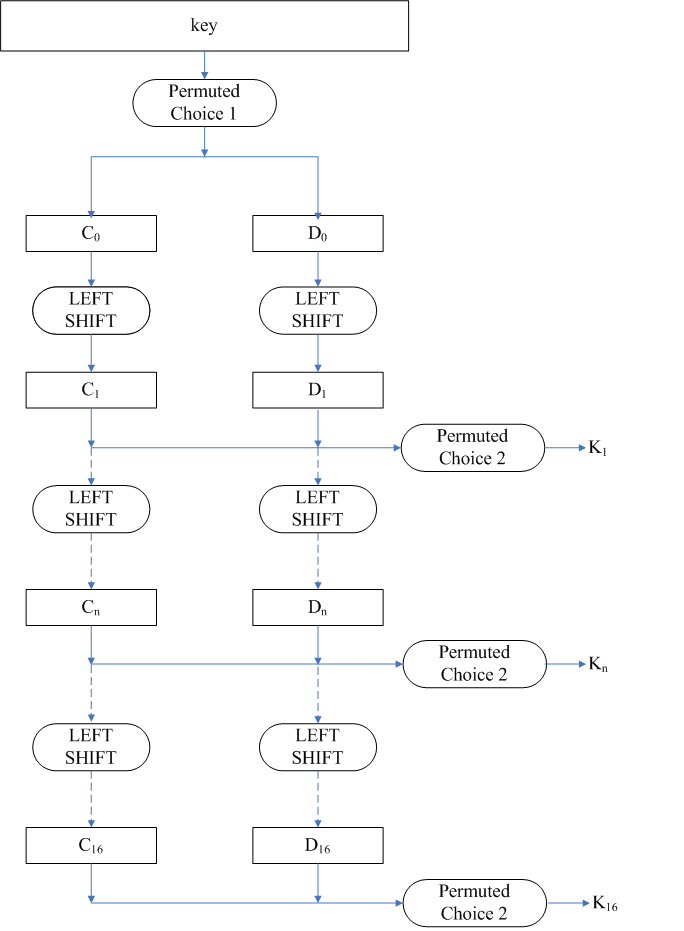
\includegraphics[scale=0.3]{../pictures/key_schedule.png}\end{center}

\begin{itemize}
	\item étape 1 : effectuer une permutation inverse $PC_{2}^{-1}(K_{16})$ afin d'obtenir $C_{16}$ et $D_{16}$.
	Il est important de noter que lors de cette permutation inverse, 8 bits sont inconnus. En effet, on passe de $48$ bits à $2 \times 28 = 56$ bits. Il y a donc 8 bits qu'on ne peut déduire à partir de $K_{16}$. \newline
	
	\begin{center}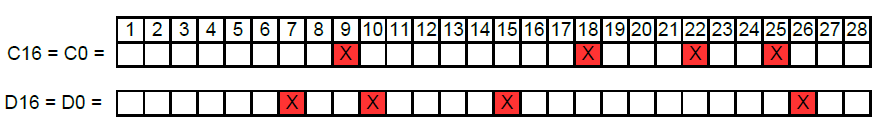
\includegraphics[scale=0.4]{../pictures/C0_D0.png}\end{center}
	
	Sur ce schéma, les bits encore inconnus sont marqués par "X". \newline
	
	
	\item étape 2 : déduire $C_{0}$ et $D_{0}$ à partir de $C_{16}$ et $D_{16}$. En effet, $C_{0}=C_{16}$ et $D_{0}=D_{16}$ puisque la somme des shifts circulaires donne $28$ qui correspond à la taille des blocs $C_i$ et $D_i$. Les 8 bits inconnus n'ont donc pas bougé de place dans $C_0$ et $D_0$. \newline
	
	\item étape 3 : effectuer une permutation inverse $PC_{1}^{-1}(C_{0}||D_{0})$ afin d'obtenir la clé finale sur 64 bits. On peut noter ici que les 8 bits inconnus sont mélangés dans la clé finale. De plus, 8 bits supplémentaires ont été rajoutés correspondant aux bits de parité. On a donc une clé finale sur 64 bits dont 16 bits sont inconnus. \newline
	
	\begin{center}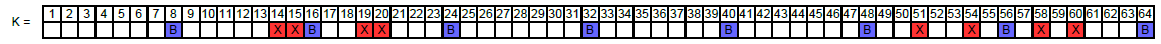
\includegraphics[scale=0.5]{../pictures/K64.png}\end{center}
	
	Sur le schéma ci-dessous, "B" correspond aux bits de parité. \newline
	
	\item étape 4 : retrouver les 8 bits inconnus par une recherche exhaustive : $2^{8}=256$ cas possibles. Pour chaque clé possible, on fait le chiffrement DES avec en entrée la clé possible et le message clair fourni. Si la clé testée est celle recherchée, alors le chiffré obtenu sera identique à celui du chiffré correct fourni. \newline
	
	\item étape 5 : déduire les 8 bits de parité en s'assurant que chaque octet possède un nombre impair de bits à 1. \newline
	
	La complexité pour trouver $K$ à partir de $K_{16}$ est de $O(2^8)$ car à partir de $K_{16}$, 8 bits sont encore inconnus pour $K$ sur 56 bits, d'où une recherche exhaustive de $O(2^8)$. A partir de cela, les 8 bits de parité (inconnus sur $K$ de 64 bits) sont à déduire en temps constant. \newline
	
	On aura donc une complexité totale pour trouver $K_{16}$ puis $K$ de $O(2^{14}+2^{8}) \simeq O(2^{14})$
	
	
\end{itemize}

\subsection{Question 2}

Après avoir implémenter les fonctions "$build\_C16\_D16$", "$build\_K56$, "$build\_K$", "$set\_parity\_bits$" et "$find\_K$" du fichier $app/src/attack.c$ fournis en annexe, on va effectuer les différentes étapes en détaillant : 

\begin{itemize}

\item On a obtenu précédemment lors de la recherche de la sous clé : $K_{16}= $ $02$ $10$ $B1$ $2C$ $47$ $79$. \newline \newline
Avec l'étape 1 et 2, on obtient : \newline 
- $C_{0}=C_{16}=$ $0110$ $00100100$ $00010000$ $00000100= 6241004$ \newline 
- $D_{0}=D_{16}=$ $0011$ $00000010$ $01001110$ $11001011= 3024ECB$ \newline
- $C_{0}||D_{0}=$ $62$ $41$ $00$ $43$ $02$ $4E$ $CB$ \newline
Les 8 bits inconnus à chercher sont à $0$. \newline

\item Avec l'étape 3, on obtient la clé DES sur 64 bits avec les 8 bits inconnus à 0 et les bits de parité également à 0 : $K_{64}*_{avant\_recherche\_exhaustive}=$ $50$ $90$ $0C$ $18$ $02$ $8E$ $D8$ $08$ \newline

\item On réalise l'attaque exhaustive et on trouve la solution en ajustant également les bits de parité et on obtient la solution finale de la clé DES sur 64 bits en hexadécimal: \newline 
\color{red}
$K_{64}=51$ $92$ $2C$ $19$ $02$ $8F$ $FD$ $49$
\color{black}

\end{itemize}

\begin{center}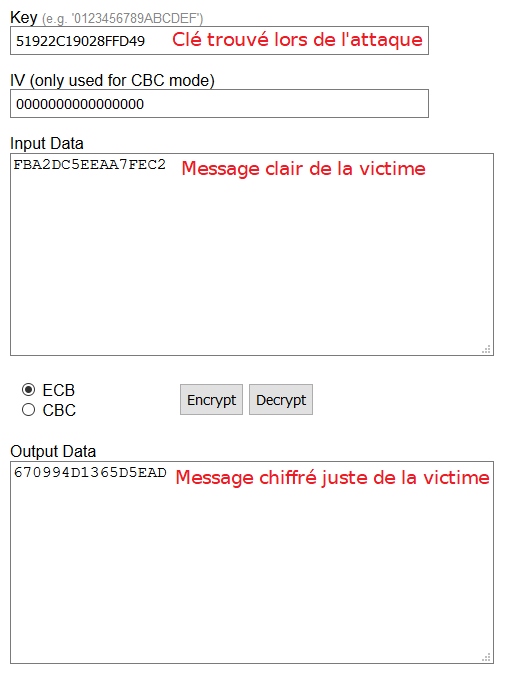
\includegraphics[scale=0.5]{../pictures/resultat.png}\end{center}

\section{Partie 4 : Fautes sur les tours précédents}

On rappelle la loi de Moore qui dit que la puissance de calcul double tous les 18 mois. Pour rendre une attaque infaisable dans le monde civil, il faudrait $2^{80}$ opérations élémentaires. \newline
De plus, nous avons trouvé une complexité de $0(2^{14})$ pour une attaque DFA sur la valeur de sortie $R_{15}$. 

\subsection{Faute provoquée sur la valeur de sortie $R_{14}$ du $14^{e}$ tour}

Pour ce type d'attaque, on obtient 2 paires d'égalités : 

\begin{itemize}
	\item $R_{15}=L_{14} \oplus f(K_{15}, R_{14})$ et $L_{15}=R_{14}$
	\item $R_{15*}=L_{14}* \oplus f(K_{15}, R_{14}*)$ et $L_{15*}=R_{14}*$
\end{itemize}

On obtient donc les équations suivantes : \newline
$R_{15} \oplus R_{15}* = L_{14} \oplus f(K_{15}, R_{14}) \oplus L_{14} \oplus f(K_{15}, R_{14}*)= f(K_{15}, R_{14}) \oplus f(K_{15}, R_{14}*)$ \newline \newline
On décompose pour obtenir $(E)$ (en rouge les valeurs inconnues et vert les valeurs connues): \newline
$P^{-1}(\color{green}R_{15}\color{black}\oplus\color{green}R_{15}*\color{black})=S_{i}(E(\color{red}R_{14}\color{black})\oplus \color{red}K_{15}\color{black})\oplus S_{i}(E(\color{red}R_{14}*\color{black})\oplus \color{red}K_{15}\color{black})$ \newline \newline
Or, $R_{14}=L_{15}=R_{16} \oplus f(K_{16}, L_{16})$ donne $P^{-1}(\color{red}L_{15}\color{black} \oplus \color{green}R_{16}\color{black})_{b_{x}\to b_{y}}=S_i(E(\color{green}L_{16}\color{black}) \oplus \color{red}K_{16}\color{black})_{b_{x}\to b_{y}}$ et \newline
$R_{14}*=L_{15}*=R_{16}* \oplus f(K_{16}, L_{16}*)$ donne $P^{-1}(\color{red}L_{15}*\color{black} \oplus \color{green}R_{16}*\color{black})_{b_{x}\to b_{y}}=S_i(E(\color{green}L_{16}*\color{black}) \oplus \color{red}K_{16}\color{black})_{b_{x}\to b_{y}}$. \newline 
On fait donc une attaque exhaustive et on déduit les valeurs possibles pour $L_{15}$ et les $L_{15}*$. Cette attaque a donc une complexité de $O(32 \times 8 \times 2^4 \times 4)=O(2^5 \times 2^3 \times 2^4 \times 2^2)=O(2^{14})$. \newline \newline
Ensuite, pour chaque $L_{15}$ et $L_{15}*$ possible, on fait une attaque de complexité de $O(2^{14})$ pour trouver $K_{15}$ avec l'équation $(E)$. \newline
On a donc une complexité de $O(2^{14} \times 2^{14})=O(2^{28})$ sur l'attaque par faute provoquée sur la valeur de sortie $R_{14}$ du $14^{e}$ tour. Cette attaque reste réaliste car sa complexité est inférieure à $O(2^{80})$.

\subsection{Faute provoquée sur la valeur de sortie $R_{i}$ du $i^{e}$ tour}

Notons $O(2^a)$ la complexité de l'attaque DFA sur DES sur la valeur de sortie de $R_{15}$. Avec le paragraphe précédent, nous avons élaboré une attaque qui fonctionne sur n'importe quelle valeur de sortie de $R_i$ en multipliant la complexité de l'attaque du tour précédent par $O(2^a)$. On obtient donc les résultats suivants : 

\begin{itemize}
	\item Pour l'attaque sur le $15^e$ tour, la complexité est de $2^{14}$, qui est une attaque réaliste. 
	\item Pour l'attaque sur le $14^e$ tour, la complexité est de $2^{28}$, qui est une attaque réaliste. 
	\item Pour l'attaque sur le $13^e$ tour, la complexité est de $2^{42}$, qui est une attaque réaliste. 
	\item Pour l'attaque sur le $12^e$ tour, la complexité est de $2^{56}$, qui est une attaque réaliste. 
	\item Pour l'attaque sur le $11^e$ tour, la complexité est de $2^{70}$, qui est encore une attaque réaliste. 
	\item Pour l'attaque sur le $10^e$ tour, la complexité est de $2^{84}$, qui est une attaque non réaliste de nos jours puisqu'elle est supérieure à $O(2^{80})$. 
	
\end{itemize}

\section{Partie 5 : Contre-mesures}

Il existe plusieurs contre-mesures possibles contre ce type d'attaque par fautes sur le DES : 
\begin{itemize}
	\item installer une sorte de "bouclier" contre les perturbations extérieures. En effet, cette attaque par faute peut être réalisée en agissant physiquement sur les composants électroniques, tels que du laser, une hausse de température ou une modification du champ magnétique environnant. Ainsi, un bouclier physique permettrait de contrer ce type d'attaque. Il n'y aura aucun impact sur le temps de calcul par rapport à une implémentation non sécurisée puisqu'on ne change pas le logiciel. Malheureusement, installer ce dispositif coûte cher et inadapté pour certains appareils. \newline
	
	\item réaliser deux fois le calcul afin de vérifier que l'on obtient deux fois le même calcul. Cela permettrait d'annuler le calcul si une attaque de ce genre était effectuée. Il y aura un impact sur le temps de calcul : vu qu'on réalisera deux fois le même calcul, alors le temps de calcul va doublé par rapport à une implémentation non sécurisée. 
\end{itemize}

\end{document}